% !TEX root = mathcraft.tex
%%%%%%%%%%%%%%%%%%%%%%%%%%%%%%%%%%%%%%%%%%%%%%%%%%%%%%%%%%%%%%%%%%%%%%%%
%%%% BEGINN EINSTELLUNG FUER DIE ARBEIT. UNBEDINGT ERFORDERLICH! %%%%%%%
%%%%%%%%%%%%%%%%%%%%%%%%%%%%%%%%%%%%%%%%%%%%%%%%%%%%%%%%%%%%%%%%%%%%%%%%
% Geben Sie Ihren Namen hier an:

\newcommand{\bearbeiter}{Luca Leon Happel}

% Herkunftsort des Bearbeiters (erscheint auf dem Deckblatt):
\newcommand{\heimatort}{Mönchengladbach}

% Geben Sie hier den Titel Ihrer Arbeit an:
\newcommand{\titel}{Mathcraft: Topos theory in videogames like minecraft}

% Falls Sie die Arbeit zweiseitig ausdrucken wollen,
% benutzen Sie die folgende Zeile mit
% \AN fuer zweiseitigen Druck
% \AUS fuer einseitigen Druck
\newcommand{\zweiseitig}{\AN}
% true fuer biber, false fuer klassischen Zitierstil
%\newcommand{\biber}{false}
\newcommand{\biber}{true}

% Falls Sections immer rechts beginnen sollen.
\newcommand{\sectionforcestartright}{false}
%\newcommand{\sectionforcestartright}{true}

% Falls die Arbeit in englischer Sprache verfasst
% werden soll, dann benutzen Sie die folgende Zeile mit
% englisch fuer englische Sprache
% deutsch fuer deutsche Sprache
\newcommand{\sprache}{englisch}


%%%%%%%%%%%%%%%%%%%%%%%%%%%%%%%%%%%%%%%%%%%%%%%%%%%%%%%%%%%%%%%%%%%%%%%%
%%%% ENDE EINSTELLUNGEN %%%%%%%%%%%%%%%%%%%%%%%%%%%%%%%%%%%%%%%%%%%%%%%%
%%%%%%%%%%%%%%%%%%%%%%%%%%%%%%%%%%%%%%%%%%%%%%%%%%%%%%%%%%%%%%%%%%%%%%%%

% Die folgende Zeile NICHT EDITIEREN oder loeschen


% !TEX root = ./mathcraft.tex
%%%%%%%%%%%%%%%%%%%%%%%%%%%%%%%%%%%%%%%%%%%%%%%%%%%%%%%%%%%
% Obere Titelmakros. Editieren Sie diese Datei nur, wenn
% Sie sich ABSOLUT sicher sind, was Sie da tun!!!
% Version 2.2 - 2.3.2010
%%%%%%%%%%%%%%%%%%%%%%%%%%%%%%%%%%%%%%%%%%%%%%%%%%%%%%%%%%%
\newcommand{\AN}{twoside}
\newcommand{\AUS}{}


%\newcommand{\englisch}{}
%\newcommand{\deutsch}{\usepackage[german]{babel}}

%% Die folgenden auskommentierten Optionen dienen der automatischen
%% Erkennung des Latex-Kompilers und dem Setzen der davon abhängigen
%% Einstellungen. Bei Problem z.B. mit dem Einbinden von verschiedenen
%% Grafiktypen bei Verwendung von PdfLatex oder Latex, einfach die
%% verschiedenen \usepackage(s) ausprobieren. (Mit diesen Einstellungen
%% funktionierte diese Vorlage bei der Verwenundg von latex.exe als
%% Kompiler bei den meisten Studierenden.)

%\newif\ifpdf \ifx\pdfoutput\undefined
%\pdffalse % we are not running pdflatex
%\else
%\pdfoutput=1 % we are running pdflatex
%\pdfcompresslevel=9 % compression level for text and image;
%\pdftrue \fi

\documentclass[11pt,a4paper, \zweiseitig]{article}
\usepackage{ifthen}


%\usepackage[iso]{umlaute}
\usepackage{iftex}
\ifPDFTeX
	\PackageError{imports}{This document must be compiled with XeLaTeX (or LuaLaTeX)}{Run xelatex (see the recipe in .vscode/settings.json or .latexmkrc), not pdflatex.}
\fi
% inputenc/fontenc are for pdfLaTeX only; XeLaTeX reads UTF-8 natively and
% fontspec replaces the OT1/T1 font-encoding machinery.
\usepackage{fontspec}
\defaultfontfeatures{Ligatures=TeX}
\setmainfont{TeX Gyre Pagella} % OpenType clone of Palatino, replaces \usepackage{palatino}
% Monospace font used for \texttt and code listings (minted below). JuliaMono
% is designed for scientific/programming use and has by far the broadest
% Unicode coverage of any monospace font (math operators, arrows, blackboard
% bold, etc.), which is exactly the symbol set used in the pseudocode in this
% document (▶, ×, ℕ, Ω, λ, ∀, ≤, ...). This lets code blocks use those symbols
% as plain UTF-8 characters instead of dropping into \mathescape.
\setmonofont{JuliaMono}[Scale=MatchLowercase]
% Fallback font for symbols/emoji outside the main font (e.g. \emoji{🌳}).
% Symbola covers a very large swath of Unicode, incl. most emoji, in outline
% (monochrome) form, which is what XeLaTeX can actually typeset; the color
% "Noto Color Emoji" font will not render in color under XeLaTeX/LuaLaTeX.
\newfontfamily\emojifont{Symbola}
\newcommand{\emoji}[1]{{\emojifont #1}}
%\usepackage{makeidx} % um ein Index zu erstellen
\usepackage[nottoc]{tocbibind}
\usepackage{fancybox} % fuer die Rahmen
\usepackage{shortvrb}
\usepackage{url}
\usepackage{xcolor}
\usepackage{nicefrac}
% minted (https://ctan.org/pkg/minted) replaces `listings`: it renders code
% via Pygments, so any Unicode symbol supported by the chosen font (see
% \setmonofont above) can be typed directly in the listing, and it produces
% much nicer highlighted/framed output ("beautiful pseudocode") than
% `listings`. It shells out to Pygments (via the `latexminted` helper), so
% compilation needs -shell-escape (already set in .latexmkrc / .vscode).
\usepackage{minted}
\usemintedstyle{bw} % Pygments "bw": bold/italic only, no color or background
\setminted{
	fontsize=\small,
	breaklines=true,
	autogobble=true, % strip common leading whitespace, so indented \begin{minted} blocks aren't shifted right
	linenos=true, % classic look: line numbers in the margin,
	frame=leftline, % separated from the code by a vertical rule
	framesep=6pt,
	numbersep=8pt,
	ignorelexererrors=true, % Pygments flags non-ASCII like ▶ as errors and draws a red box around them
	baselinestretch=1.2,
}
\renewcommand{\theFancyVerbLine}{\scriptsize\arabic{FancyVerbLine}}
\setlength{\marginparwidth}{2cm}
\usepackage{todonotes}
\usepackage{enumitem} % (a), (b), ... labels in definitions
\usepackage[colorlinks,citecolor=black,linkcolor=black,urlcolor=black]{hyperref} %anklickbares Inhaltsverzeichnis

\ifthenelse{\equal{\biber}{true}}{
	% only needed for biber
	\usepackage{csquotes}
	\usepackage[style=numeric,sorting=none,natbib=true,backend=biber,mincitenames=1,maxcitenames=2,maxbibnames=99,uniquelist=false]{biblatex}

	% https://tex.stackexchange.com/a/334703/8850
	\AtEveryBibitem{%
		\clearfield{issn}
		\clearfield{isbn}
		\clearfield{doi}
		\clearfield{location}
		\clearlist{location}
		\clearlist{address}

		\ifentrytype{online}{}{% Remove url except for @online and @thesis
			\ifentrytype{thesis}{}{\clearfield{url}}
		}
	}
}
{}%no else

% Falls es bei \citet ein Komma zwischen Name und Jahr gibt:
% https://tex.stackexchange.com/questions/312539/unwanted-comma-between-author-and-year-using-citet-command
% (thx @ Markus Brenneis)
%\DeclareDelimFormat[cbx@textcite]{nameyeardelim}{\addspace}



\ifthenelse{\equal{\sprache}{deutsch}}{
	\usepackage[ngerman]{babel}
	% Bibtex u.a -> et al.
	\ifthenelse{\equal{\biber}{true}}{
		\DefineBibliographyStrings{ngerman}{
			andothers = {{et\,al\adddot}},
		}
		\newcommand{\references}{Literatur}
	}
	{} % do nothing when not using biber
	\usepackage[autostyle, german=quotes]{csquotes} % Deutsche Anführungszeichen im Literaturverzeichnis (thx @ Markus Brenneis)

}{ \newcommand{\references}{References}}

\usepackage{a4wide} % ganze A4 Weite verwenden



%\ifpdf
%\usepackage[pdftex,xdvi]{graphicx}
%\usepackage{thumbpdf} %thumbs fuer Pdf
%\usepackage[pdfstartview=FitV]{hyperref} %anklickbares Inhaltsverzeichnis
%\else
%\usepackage[dvips,xdvi]{graphicx}
\usepackage{graphicx}
\usepackage{caption}
\usepackage{subcaption}
\usepackage[section]{placeins} % floats stay within their section
\usepackage{array}
\usepackage{booktabs}

%\fi

% Mathematik / kategorientheoretische Notation und kommutative Diagramme
\usepackage{amsmath}
\usepackage{mathtools} % \coloneqq
\usepackage{amssymb}
\usepackage{amsthm}
\usepackage{stmaryrd} % \llbracket, \rrbracket
\usepackage{tikz-cd}
\usepackage{tikz-3dplot}
\usepackage{pgfplots}
\usepackage[super]{nth}
\pgfplotsset{compat=1.18}
\usetikzlibrary{3d, positioning, arrows.meta, patterns, patterns.meta}
% chains of nodes drawn by the forests F(U_m) of the elements U_m of \Omega(n)
\tikzset{forestrow/.style={baseline=-0.5ex, x=0.6cm, >=Stealth},
	onode/.style={draw, rounded corners=3pt, fill=white, inner sep=1pt,
			font=\scriptsize, minimum width=4mm, minimum height=3.5mm},
	oedge/.style={->, thin}}
% \forestchain{0,1,\cdots,n}: a chain of labeled nodes, each pointing to its
% left neighbour; a \cdots entry is drawn without a box
\def\forestchaindots{\cdots}
\newcommand{\forestchain}[1]{\tikz[forestrow]{%
		\foreach \l [count=\i, remember=\i as \j (initially 0)] in {#1} {%
				\ifx\l\forestchaindots \tikzset{chainnode/.style={inner sep=0pt}}%
				\else \tikzset{chainnode/.style={onode}}\fi
				\ifnum\i=1 \node[chainnode] (v\i) at (0, 0) {$\l$};%
				\else \node[chainnode, right=1.8mm of v\j] (v\i) {$\l$}; \draw[oedge] (v\i) -- (v\j);\fi
			}}}
% inline glyphs for the node labels of the graphs in Fig.~\ref{fig:lattices},
% drawn like the nodes there: a cube, a face, an edge and a vertex
\tikzset{cellglyphpic/.style={x={(1.0cm,0cm)}, y={(0.55cm,0.38cm)}, z={(0cm,1.0cm)},
			scale=0.26, line join=round, line cap=round, baseline=0.1ex},
	inlinecellglyph/.style={line width=0.45pt, preaction={fill=white}}}
\newcommand{\cubeglyph}{\tikz[cellglyphpic]{%
		\draw[inlinecellglyph] (0,0,0) -- (1,0,0) -- (1,0,1) -- (0,0,1) -- cycle;
		\draw[inlinecellglyph, pattern={Lines[angle=90, distance=1.1pt, line width=0.3pt]}]
		(1,0,0) -- (1,1,0) -- (1,1,1) -- (1,0,1) -- cycle;
		\draw[inlinecellglyph, pattern={Dots[distance=1.2pt, radius=0.3pt]}]
		(0,0,1) -- (1,0,1) -- (1,1,1) -- (0,1,1) -- cycle;}}
\newcommand{\faceglyph}{\tikz[cellglyphpic]{%
		\draw[inlinecellglyph] (0,0,0) -- (1,0,0) -- (1,0,1) -- (0,0,1) -- cycle;}}
\newcommand{\edgeglyph}{\tikz[cellglyphpic]{%
		\draw[line width=2.6pt, line cap=round] (0,0,0.5) -- (1,0,0.5);
		\draw[line width=1.4pt, line cap=round, white] (0,0,0.5) -- (1,0,0.5);}}
\newcommand{\vertexglyph}{\tikz[baseline=0.1ex]{%
		\draw[inlinecellglyph] (0,0.13cm) circle[radius=2.2pt];}}
\usepackage{mathpartir} % inference rules for the internal logic
\usepackage{aliascnt}
\usepackage[capitalise,nameinlink]{cleveref}

\newtheorem{theorem}{Theorem}[section]
% each environment gets an alias of the theorem counter, so that the shared
% numbering is kept but cleveref sees the environment name, not "theorem"
\newcommand{\newsharedtheorem}[2]{%
	\newaliascnt{#1}{theorem}%
	\newtheorem{#1}[#1]{#2}%
	\aliascntresetthe{#1}}
\newsharedtheorem{definition}{Definition}
\newsharedtheorem{proposition}{Proposition}
\newsharedtheorem{lemma}{Lemma}
\newsharedtheorem{corollary}{Corollary}
\newsharedtheorem{example}{Example}
\newsharedtheorem{remark}{Remark}

\newcommand{\Set}{\mathbf{Set}}
\newcommand{\Top}{\mathbf{Top}}
\newcommand{\functorcat}[2]{[#1,\, #2]}
\newcommand{\toposoftrees}{\mathcal{S}}
\newcommand{\toposofgraphs}{\mathcal{G}}
\newcommand{\restr}[2]{#1|_{#2}}
\newcommand{\Sub}[1]{\mathrm{Sub}_{#1}}
\newcommand{\NN}{\mathbb{N}}
\newcommand{\ZZ}{\mathbb{Z}}
\newcommand{\RR}{\mathbb{R}}
\newcommand{\CC}{\mathbb{C}}
\newcommand{\Stream}{\texttt{Str}}
\newcommand{\List}{\mathrm{List}}
\newcommand{\Blocks}{\mathrm{Blocks}}
\newcommand{\Entities}{\mathrm{Entities}}
\newcommand{\BlockID}{\mathrm{BlockID}}
\newcommand{\EntityID}{\mathrm{EntityID}}
\newcommand{\Hom}{\text{Hom}}
\newcommand{\Nat}{\text{Nat}}
\newcommand{\StreamG}{\Stream}
\newcommand{\StreamedTreeG}{\texttt{StrTree}}
\newcommand{\BinTreeG}{\texttt{Tree}}
\newcommand{\im}{\text{im }}
\newcommand{\treeEmbedding}{F}
\newcommand{\later}{\mathord{\blacktriangleright}}
\newcommand{\before}{\mathord{\blacktriangleleft}}
\newcommand{\laterModal}{\triangleright}
\newcommand{\alwaysModal}{\Box}
\newcommand{\eventuallyModal}{\Diamond}
\newcommand{\liftingMonad}{L}
\newcommand{\laterT}{\triangleright}
\newcommand{\fixLater}{\text{fix}}
% semantic brackets for the interpretation of the internal language
\newcommand{\sem}[1]{[\![#1]\!]}
\newcommand{\id}{\text{id}}
\newcommand{\avg}{\text{avg}}
\newcommand{\true}{\text{true}}
\newcommand{\false}{\text{false}}
\newcommand{\Hask}{\mathbf{Hask}}
\newcommand{\Bool}{\text{Bool}}
\newcommand{\RForest}{\mathbf{RForest}}
% Signature components as in the Elephant (D1.1.1); optional argument is the signature
\newcommand{\SigType}[1][\Sigma]{#1\text{-}\mathrm{Type}}
\newcommand{\SigFun}[1][\Sigma]{#1\text{-}\mathrm{Fun}}
\newcommand{\SigRel}[1][\Sigma]{#1\text{-}\mathrm{Rel}}
\newcommand{\SigTerm}[1][\Sigma]{#1\text{-}\mathrm{Term}}
\newcommand{\SigForm}[1][\Sigma]{#1\text{-}\mathrm{Form}}

\newcommand{\redt}[1] {
	\textcolor{red}{#1}}

\newcommand{\oranget}[1] {
	\textcolor{orange}{#1}}

\newcommand{\purplet}[1] {
	\textcolor{purple}{#1}}

%%%%%%%%%%%%%%%%%%%%%%% Massangaben fuer die Arbeit %%%%%%%%%%%%%%%
\setlength{\textwidth}{15cm}

\setlength{\oddsidemargin}{35mm}
\setlength{\evensidemargin}{25mm}

\addtolength{\oddsidemargin}{-1in}
\addtolength{\evensidemargin}{-1in}

\ifthenelse{\equal{\biber}{true}}{\addbibresource{references.bib}}{}

%\makeindex

\begin{document}
%\setcounter{secnumdepth}{4} %Nummerieren bis in die 4. Ebene
%\setcounter{tocdepth}{4} %Inhaltsverzeichnis bis zur 4. Ebene

\pagestyle{headings}

\sloppy % LaTeX ist dann nicht so streng mit der Silbentrennung
%~ \MakeShortVerb{\§}

\parindent0mm
\parskip0.5em


{
\textwidth170mm
\oddsidemargin30mm
\evensidemargin30mm
\addtolength{\oddsidemargin}{-1in}
\addtolength{\evensidemargin}{-1in}

\parskip0pt plus2pt

% Die Raender muessen eventuell fuer jeden Drucker individuell eingestellt
% werden. Dazu sind die Werte fuer die Abstaende `\oben' und `\links' zu
% aendern, die von mir auf jeweils 0mm eingestellt wurden.

%\newlength{\links} \setlength{\links}{10mm}  % hier abzuaendern
%\addtolength{\oddsidemargin}{\links}
%\addtolength{\evensidemargin}{\links}

% draft warning: a page-filling red exclamation mark with "DRAFT" below it
\begin{titlepage}
	\vspace*{\fill}
	\begin{center}
		
\begin{tikzpicture}[scale=0.9]
			\fill[red, rounded corners=8mm]
			(-2.2, 0) -- (2.2, 0) -- (1.2, -13) -- (-1.2, -13) -- cycle;
			\fill[red] (0, -15.8) circle[radius=1.7];
			\node[text=red, font=\bfseries, anchor=north] at (0, -18.2)
			{\resizebox{11cm}{!}{DRAFT}};
		\end{tikzpicture}
	\end{center}
	\vspace*{\fill}
\end{titlepage}

\begin{titlepage}
	\vspace*{14em}

	% Titel
	\begin{center}
		\baselineskip=55pt
		\textbf{\huge \titel}
		\baselineskip=0 pt
	\end{center}

	%\vspace{7em}

	\vfill

	% Autor
	\begin{center}
		\textbf{\Large
			\bearbeiter
		}

		\vspace{1em}
		from \heimatort
	\end{center}

\end{titlepage}

}

%%%%%%%%%%%%%%%%%%%%%%%%%%%%%%%%%%%%%%%%%%%%%%%%%%%%%%%%%%%%%%%%%%%%%
\clearpage
\begin{titlepage}
	~                % eine leere Seite hinter dem Deckblatt
\end{titlepage}
%%%%%%%%%%%%%%%%%%%%%%%%%%%%%%%%%%%%%%%%%%%%%%%%%%%%%%%%%%%%%%%%%%%%%
\clearpage
\begin{titlepage}

	%%% Die folgende Zeile nicht ändern!
\section*{Acknowledgements}
%%% Danksagung:
% TODO



	%%%%%%%%%%%%%%%%%%%%%%%%%%%%%%%%%%%%%%%%%%%%%%%%
	% Untere Titelmakros. Editieren Sie diese Datei nur, wenn Sie sich
	% ABSOLUT sicher sind, was Sie da tun!!!
	%%%%%%%%%%%%%%%%%%%%%%%%%%%%%%%%%%%%%%%%%%%%%%%
	\vspace*{\fill}
\end{titlepage}

%%%%%%%%%%%%%%%%%%%%%%%%%%%%%%%%%%%%%%%%%%%%%%%%%%%%%%%%%%%%%%%%%%%%%
% Leerseite bei zweiseitigem Druck
%%%%%%%%%%%%%%%%%%%%%%%%%%%%%%%%%%%%%%%%%%%%%%%%%%%%%%%%%%%%%%%%%%%%%
\ifthenelse{\equal{\zweiseitig}{twoside}}
{\clearpage\begin{titlepage}~\end{titlepage}}{}
%%%%%%%%%%%%%%%%%%%%%%%%%%%%%%%%%%%%%%%%%%%%%%%%%%%%%%%%%%%%%%%%%%%%%
\clearpage \setcounter{page}{1}
\pagenumbering{roman}
\setcounter{tocdepth}{2}
\tableofcontents

%\enlargethispage{\baselineskip}
\clearpage
%%%%%%%%%%%%%%%%%%%%%%%%%%%%%%%%%%%%%%%%%%%%%%%%%%%%%%%%%%%%%%%%%%%%%
% Leere Seite, falls Inhaltsverzeichnis mit ungerader Seitenzahl und
% doppelseitiger Druck
%%%%%%%%%%%%%%%%%%%%%%%%%%%%%%%%%%%%%%%%%%%%%%%%%%%%%%%%%%%%%%%%%%%%%
\ifthenelse{ \( \equal{\zweiseitig}{twoside} \and \not \isodd{\value{page}} \)}
{\pagebreak \thispagestyle{empty} \cleardoublepage}{\clearpage}


% Kapitel soll bei doppelseitigem Druck immer auf der rechten (ungeraden) Seite anfangen (thx @ Philipp Grawe)
% https://tex.stackexchange.com/a/223387
\ifthenelse{\boolean{\sectionforcestartright}}
{\let\oldsection\section % Store \section in \oldsection
	\renewcommand{\section}{\cleardoublepage\oldsection}}
{}

\pagenumbering{arabic}
\setcounter{page}{1}

%%%%%%%%%%%%%%%%%%%%%%%%%%%%%%%%%%%%%%%%%%%%%%%%%%%%%%%%%%%%%%%%%%%%%%%%
%%%% BEGINN TEXTTEIL %%%%%%%%%%%%%%%%%%%%%%%%%%%%%%%%%%%%%%%%%%%%%%%%%%%
%%%%%%%%%%%%%%%%%%%%%%%%%%%%%%%%%%%%%%%%%%%%%%%%%%%%%%%%%%%%%%%%%%%%%%%%

%%%%%%%%%%%%%%%%%%%%%%%%%%%%%%%%%%%%%%%%%%%%%%%%%%%%%%%%%%%%%%%%%%%%%%%%
% Text entweder direkt hier hinein schreiben oder, im Sinne der
% besseren Uebersichtlich- und Bearbeitbarkeit mittels \input die
% einzelnen Textteile hier einbinden.
%%%%%%%%%%%%%%%%%%%%%%%%%%%%%%%%%%%%%%%%%%%%%%%%%%%%%%%%%%%%%%%%%%%%%%%%

\section{Introduction}\label{sec:introduction}

As established in \cite{happelSheavesMinecraft2021}, information that depends
on location can be modelled using \emph{sheaves}. We wish to expand on this idea
in the context of the popular video game \emph{Minecraft}. Its world is a subset
of $\RR^3$, inhabited by two kinds of objects:
\begin{enumerate}[label=(\arabic*)]
	\item \emph{blocks}, which are unit cubes placed on the lattice
	      $\ZZ^3 \subset \RR^3$, and
	\item \emph{entities}, such as dropped items, players and enemies. Several
	      entities may occupy the same location at the same time.
\end{enumerate}

To render a (more or less) infinite world in finite time, Minecraft
approximates it by finitely many pieces, a technique known as
\emph{chunking}. A \emph{chunk} is a bounded region of $\RR^3$, together with
the information about which blocks and which entities are placed inside of it.
In \cite{happelSheavesMinecraft2021} we saw that chunking can in fact be
modelled using (pre)sheaves. To this end, fix a width $w$, a depth $d$ and a
height $h$, all positive integers, and equip $\RR^3$ with the topology $\tau$
generated by the closed boxes
\[
	C_{i,j,k}^{w,d,h} = [i, i+w] \times [j, j+d] \times [k, k+h],
	\qquad (i,j,k) \in w\ZZ \times d\ZZ \times h\ZZ.
\]
These boxes tile the space $\RR^3$, as seen in \cref{fig:chunk-tiling}. Since
the boxes are closed, two neighbouring chunks share a common face, so $\tau$
contains not only (unions of) chunks but also their faces, edges and vertices
as open sets.

\begin{figure}[ht]
	\centering
	\begin{tikzpicture}[
			x={(1.0cm,0cm)}, y={(0.55cm,0.38cm)}, z={(0cm,1.0cm)},
			scale=1.15, line join=round, line cap=round,
			grid/.style={line width=0.5pt},
			stub/.style={line width=0.4pt, dash pattern=on 1.5pt off 1.5pt},
		]
		% chunk dimensions (in picture units) and number of chunks shown
		\def\w{1}\def\d{1}\def\h{1.25}
		\def\nx{4}\def\ny{3}\def\nz{2}
		\pgfmathsetmacro{\X}{\nx*\w}
		\pgfmathsetmacro{\Y}{\ny*\d}
		\pgfmathsetmacro{\Z}{\nz*\h}

		% faces of the block, shaded by ordered dithering (black/white only)
		\fill[white] (0,0,0) -- (\X,0,0) -- (\X,0,\Z) -- (0,0,\Z) -- cycle;
		\fill[pattern=dots] (0,0,\Z) -- (\X,0,\Z) -- (\X,\Y,\Z) -- (0,\Y,\Z) -- cycle;
		\fill[pattern=crosshatch dots] (\X,0,0) -- (\X,\Y,0) -- (\X,\Y,\Z) -- (\X,0,\Z) -- cycle;

		% one distinguished chunk C_{0,0,h}^{w,d,h} on the front face
		\fill[pattern=north east lines] (\w,0,\h) -- (2*\w,0,\h) -- (2*\w,0,2*\h) -- (\w,0,2*\h) -- cycle;

		% grid lines on the three visible faces
		\foreach \i in {0,...,\nx} {
				\draw[grid] (\i*\w,0,0) -- (\i*\w,0,\Z) -- (\i*\w,\Y,\Z);
				\draw[stub] (\i*\w,0,0) -- (\i*\w,0,-0.45);
				\draw[stub] (\i*\w,\Y,\Z) -- (\i*\w,\Y+0.8,\Z);
			}
		\foreach \k in {0,...,\nz} {
				\draw[grid] (0,0,\k*\h) -- (\X,0,\k*\h) -- (\X,\Y,\k*\h);
				\draw[stub] (0,0,\k*\h) -- (-0.45,0,\k*\h);
				\draw[stub] (\X,\Y,\k*\h) -- (\X,\Y+0.8,\k*\h);
			}
		\foreach \j in {0,...,\ny} {
				\draw[grid] (0,\j*\d,\Z) -- (\X,\j*\d,\Z) -- (\X,\j*\d,0);
				\draw[stub] (0,\j*\d,\Z) -- (-0.45,\j*\d,\Z);
				\draw[stub] (\X,\j*\d,0) -- (\X,\j*\d,-0.45);
			}

		% outline
		\draw[line width=0.9pt] (0,0,0) -- (\X,0,0) -- (\X,\Y,0) -- (\X,\Y,\Z)
		-- (0,\Y,\Z) -- (0,0,\Z) -- cycle;
		\draw[line width=0.9pt] (0,0,\Z) -- (\X,0,\Z) -- (\X,\Y,\Z);
		\draw[line width=0.9pt] (\X,0,0) -- (\X,0,\Z);

		% dimensions of a single chunk
		\draw[{Bar[width=4pt]}-{Bar[width=4pt]}, line width=0.4pt]
		(0,0,-0.75) -- node[fill=white, inner sep=1.5pt] {$w$} (\w,0,-0.75);
		\draw[{Bar[width=4pt]}-{Bar[width=4pt]}, line width=0.4pt]
		(\X+0.55,0,-0.1) -- node[below right=-1pt, inner sep=1.5pt] {$d$} (\X+0.55,\d,-0.1);
		\draw[{Bar[width=4pt]}-{Bar[width=4pt]}, line width=0.4pt]
		(-0.85,0,0) -- node[fill=white, inner sep=1.5pt] {$h$} (-0.85,0,\h);

		% label of the distinguished chunk
		\node[fill=white, inner sep=1.5pt, font=\small] at (1.5*\w,0,1.5*\h) {$C_{w,0,h}^{w,d,h}$};
	\end{tikzpicture}
	\caption{The boxes $C_{i,j,k}^{w,d,h}$ tile the space $\RR^3$. Only finitely many
		chunks are drawn. The dashed lines indicate that the tiling continues
		in every direction.}
	\label{fig:chunk-tiling}
\end{figure}

A sheaf over chunks is then given by a contravariant functor
$P \colon \tau^{\mathrm{op}} \to \Set$, which assigns to every chunk the set
\[
	P(C_{i,j,k}^{w,d,h}) = \Blocks_{w,d,h} \times \Entities_{w,d,h}
\]
of its possible contents, where
\begin{align*}
	\Blocks_{w,d,h}   & \coloneqq \Hom_{\Set}(\NN_{<w} \times \NN_{<d} \times \NN_{<h},\ \Block), \\
	\Entities_{w,d,h} & \coloneqq \Hom_{\Set}([0,w) \times [0,d) \times [0,h),\ \List(\Entity)),
\end{align*}
where $\Block$ is the set of all possible blocks (say
$\mathrm{AirBlock} \in \Block$, $\mathrm{DirtBlock} \in \Block$,
$\mathrm{WaterBlock} \in \Block$, and so on), and $\Entity$ is the set of all
possible entities (say $\mathrm{Player} \in \Entity$,
$\mathrm{Zombie} \in \Entity$, and so on). A function in $\Blocks_{w,d,h}$
assigns a block to every position of a chunk, and a function in
$\Entities_{w,d,h}$ assigns to every point of a chunk the entities located
there. Here $\List(A)$ is the inductive set with
$\List(A) \cong A \times \List(A) + 1$. Since the value at a point is a list,
multiple entities may share a position.

Crucially, $P$ needs to satisfy the \emph{sheaf conditions}, so for every open
set $U$ and every open cover $U = \bigcup_{\iota \in I} U_\iota$,
\begin{enumerate}[label=(\roman*)]
	\item \emph{locality}: if $s, t \in P(U)$ satisfy
	      $\restr{s}{U_\iota} = \restr{t}{U_\iota}$ for all $\iota \in I$, then
	      $s = t$, and
	\item \emph{gluing}: if $s_\iota \in P(U_\iota)$ is a family with
	      $\restr{s_\iota}{U_\iota \cap U_\kappa} = \restr{s_\kappa}{U_\iota \cap U_\kappa}$
	      for all $\iota, \kappa \in I$, then there is some $s \in P(U)$ with
	      $\restr{s}{U_\iota} = s_\iota$ for all $\iota \in I$.
\end{enumerate}
These conditions are important because for the boundaries between chunks they
ensure that two neighbouring chunks, which share a common face, fit together.
For further information about the need for these conditions, consider
\cite{happelSheavesMinecraft2021}.

We may also obtain $P$ as the product $P = E \times B$ of an \emph{entity
	sheaf} $E$ and a \emph{block sheaf} $B$, with $E(C_{i,j,k}^{w,d,h}) = \Entities_{w,d,h}$
and $B(C_{i,j,k}^{w,d,h}) = \Blocks_{w,d,h}$. This works because a functor into a product
of categories is the same as a pair of functors,
\[
	\functorcat{\tau^{\mathrm{op}}}{\Set \times \Set}
	\cong \functorcat{\tau^{\mathrm{op}}}{\Set} \times \functorcat{\tau^{\mathrm{op}}}{\Set},
\]
\todo[inline]{Is this really true for sheaves?}
and $P$ is the image of the pair $(B, E)$ under this isomorphism, composed with
the product functor ${\times} \colon \Set \times \Set \to \Set$.

\begin{figure}[ht]
	\centering
	% ----------------------------------------------------------------
	% Shared drawing code (local to this figure).
	% Same parallel projection as in Fig.~\ref{fig:chunk-tiling}.
	% ----------------------------------------------------------------
	\tikzset{
		sheafpic/.style={
				x={(1.0cm,0cm)}, y={(0.55cm,0.38cm)}, z={(0cm,1.0cm)},
				scale=0.98, line join=round, line cap=round},
		chunkline/.style={line width=0.4pt, dash pattern=on 2pt off 1.5pt},
		chunkstub/.style={line width=0.3pt, dash pattern=on 0.8pt off 1.6pt},
		vox/.style={line width=0.3pt, preaction={fill=white}},
		% ordered "dithering": black and white only
		dither sparse/.style={pattern={Dots[distance=2.2pt, radius=0.28pt]}},
		dither mid/.style={pattern={Dots[distance=1.3pt, radius=0.3pt]}},
		dither lines/.style={pattern={Lines[angle=45, distance=1.3pt, line width=0.3pt]}},
		dither vert/.style={pattern={Lines[angle=90, distance=1.1pt, line width=0.3pt]}},
		dither dark/.style={pattern={Hatch[angle=45, distance=1.1pt, line width=0.3pt]}},
	}
	% a unit cube at voxel (#1,#2,#3), faces styled #4 (top), #5 (front), #6 (right)
	\newcommand{\vox}[6]{%
		\draw[vox,#5] (#1,#2,#3) -- ++(1,0,0) -- ++(0,0,1) -- ++(-1,0,0) -- cycle;
		\draw[vox,#6] ({#1+1},#2,#3) -- ++(0,1,0) -- ++(0,0,1) -- ++(0,-1,0) -- cycle;
		\draw[vox,#4] (#1,#2,{#3+1}) -- ++(1,0,0) -- ++(0,1,0) -- ++(-1,0,0) -- cycle;}
	\newcommand{\dirt}[3]{\vox{#1}{#2}{#3}{dither sparse}{dither mid}{dither dark}}
	\newcommand{\grass}[3]{\vox{#1}{#2}{#3}{dither sparse}{dither mid}{dither dark}}
	\newcommand{\wood}[3]{\vox{#1}{#2}{#3}{dither mid}{dither vert}{dither dark}}
	\newcommand{\leaves}[3]{\vox{#1}{#2}{#3}{dither sparse}{dither lines}{dither dark}}
	\newcommand{\chest}[3]{%
		\begin{scope}[shift={({#1+0.1},{#2+0.1},#3)}, scale=0.8]
			\vox{0}{0}{0}{}{}{dither sparse}
			\draw[line width=0.3pt] (0,0,0.62) -- (1,0,0.62) -- (1,1,0.62);
			\fill (0.42,0,0.48) rectangle (0.58,0,0.72);
		\end{scope}}
	% the chunk grid of Fig.~\ref{fig:chunk-tiling}, outlined by dashed lines only
	\newcommand{\chunkgrid}{%
		\def\w{1}\def\d{1}\def\h{1.25}
		\def\nx{4}\def\ny{3}\def\nz{2}
		\pgfmathsetmacro{\X}{\nx*\w}
		\pgfmathsetmacro{\Y}{\ny*\d}
		\pgfmathsetmacro{\Z}{\nz*\h}
		\foreach \i in {0,...,\nx} {
				\draw[chunkline] (\i*\w,0,0) -- (\i*\w,0,\Z) -- (\i*\w,\Y,\Z);
				\draw[chunkstub] (\i*\w,0,0) -- (\i*\w,0,-0.45);
				\draw[chunkstub] (\i*\w,\Y,\Z) -- (\i*\w,\Y+0.6,\Z);
			}
		\foreach \k in {0,...,\nz} {
				\draw[chunkline] (0,0,\k*\h) -- (\X,0,\k*\h) -- (\X,\Y,\k*\h);
				\draw[chunkstub] (0,0,\k*\h) -- (-0.45,0,\k*\h);
				\draw[chunkstub] (\X,\Y,\k*\h) -- (\X,\Y+0.6,\k*\h);
			}
		\foreach \j in {0,...,\ny} {
				\draw[chunkline] (0,\j*\d,\Z) -- (\X,\j*\d,\Z) -- (\X,\j*\d,0);
				\draw[chunkstub] (0,\j*\d,\Z) -- (-0.45,\j*\d,\Z);
				\draw[chunkstub] (\X,\j*\d,0) -- (\X,\j*\d,-0.45);
			}
		% hidden edges of the distinguished chunk C_{w,0,h}^{w,d,h}
		\draw[chunkline] (\w,\d,\h) -- (2*\w,\d,\h);
		\draw[chunkline] (\w,0,\h) -- (\w,\d,\h) -- (\w,\d,2*\h);
		\draw[chunkline] (2*\w,0,\h) -- (2*\w,\d,\h) -- (2*\w,\d,2*\h);
		% dimensions of a single chunk
		\draw[{Bar[width=4pt]}-{Bar[width=4pt]}, line width=0.4pt]
		(0,0,-0.75) -- node[fill=white, inner sep=1.5pt] {$w$} (\w,0,-0.75);
		\draw[{Bar[width=4pt]}-{Bar[width=4pt]}, line width=0.4pt]
		(\X+0.55,0,-0.1) -- node[below right=-1pt, inner sep=1.5pt] {$d$} (\X+0.55,\d,-0.1);
		\draw[{Bar[width=4pt]}-{Bar[width=4pt]}, line width=0.4pt]
		(-0.85,0,0) -- node[fill=white, inner sep=1.5pt] {$h$} (-0.85,0,\h);
	}
	% voxel coordinates inside C_{w,0,h}^{w,d,h}: 5 x 5 x 6 cubes of side 0.2
	\tikzset{inchunk/.style={shift={(1.1,0,1.25+0.025)}, scale=0.2}}
	\begin{subfigure}[b]{0.49\textwidth}
		\centering
		\begin{tikzpicture}[sheafpic]
			\chunkgrid
			\begin{scope}[inchunk]
				\leaves{0}{4}{4}
\leaves{1}{4}{4}
\leaves{1}{4}{5}
\leaves{2}{4}{4}
\dirt{0}{3}{0}
\grass{0}{3}{1}
\leaves{0}{3}{4}
\leaves{0}{3}{5}
\dirt{1}{3}{0}
\grass{1}{3}{1}
\wood{1}{3}{2}
\wood{1}{3}{3}
\leaves{1}{3}{4}
\leaves{1}{3}{5}
\leaves{2}{3}{4}
\leaves{2}{3}{5}
\dirt{0}{2}{0}
\grass{0}{2}{1}
\leaves{0}{2}{4}
\dirt{1}{2}{0}
\grass{1}{2}{1}
\leaves{1}{2}{4}
\leaves{1}{2}{5}
\leaves{2}{2}{4}
\dirt{0}{1}{0}
\grass{0}{1}{1}
\dirt{1}{1}{0}
\grass{1}{1}{1}
\dirt{2}{1}{0}
\grass{2}{1}{1}
\dirt{3}{1}{0}
\grass{3}{1}{1}
\dirt{0}{0}{0}
\grass{0}{0}{1}
\dirt{1}{0}{0}
\grass{1}{0}{1}
\dirt{2}{0}{0}
\grass{2}{0}{1}
\dirt{3}{0}{0}
\grass{3}{0}{1}
\chest{3}{0}{2}
			\end{scope}
			% front edges of C_{w,0,h}^{w,d,h} lie in front of the island
			\draw[chunkline] (1,0,1.25) rectangle (2,0,2.5);
		\end{tikzpicture}
		\caption{The block sheaf $B$: blocks placed in the chunk $C_{w,0,h}^{w,d,h}$.}
		\label{fig:block-sheaf}
	\end{subfigure}%
	\hfill
	\begin{subfigure}[b]{0.49\textwidth}
		\centering
		\begin{tikzpicture}[sheafpic]
			\chunkgrid
			\begin{scope}[inchunk]
				% a player standing where the island's grass would be
				\fill (2.6,0.5,2) circle[radius=0.12];
				\begin{scope}[shift={(2.6,0.5,2)}, line width=0.5pt]
					\draw (-0.3cm,0cm) -- (0cm,0.8cm) -- (0.3cm,0cm);
					\draw (0cm,0.8cm) -- (0cm,1.45cm);
					\draw (-0.45cm,0.9cm) -- (0cm,1.3cm) -- (0.45cm,0.9cm);
					\draw[preaction={fill=white}] (0cm,1.67cm) circle[radius=0.22cm];
				\end{scope}
			\end{scope}
		\end{tikzpicture}
		\caption{The entity sheaf $E$: a player standing in the chunk $C_{w,0,h}^{w,d,h}$.}
		\label{fig:entity-sheaf}
	\end{subfigure}
	\caption{The two components of $P = E \times B$ over the same chunk
		$C_{w,0,h}^{w,d,h}$. Blocks (left) sit on the lattice $\ZZ^3$, entities (right)
		at arbitrary points.}
	\label{fig:block-entity-sheaf}
\end{figure}

The topology $\tau$ induces a labelled graph $\gamma$. For each chunk, we add a
node labelled by \cubeglyph, and for their faces we add nodes labelled by
\faceglyph, and similarly for their edges \edgeglyph{} and vertices
\vertexglyph. These nodes are then connected by edges iff one of the two
corresponding cells lies on the boundary of the other, where each edge needs to
join cells of consecutive dimensions, that is, a chunk \cubeglyph{} with a face
\faceglyph, a face \faceglyph{} with an edge \edgeglyph, or an edge
\edgeglyph{} with a vertex \vertexglyph.

We call a sheaf $P \colon \tau^{\mathrm{op}} \to \Set$ with
$P(C_{i,j,k}^{w,d,h}) = \Blocks_{w,d,h} \times \Entities_{w,d,h}$ a \emph{Euclidean
	Mathcraft sheaf}. This would yield the induced labelled graph $X$ in
\cref{fig:chunk-lattice}. We could also consider other topologies which also
yield such a labelled graph, like one that induces the graph $Y$ as shown in
\cref{fig:wormhole-lattice}, where we added a \enquote{wormhole}, which is
given by an additional face \faceglyph{} shared by two chunks \cubeglyph. This
justifies the term \emph{Euclidean} to distinguish between the standard
topology and others.

\begin{figure}[ht]
	\centering
	\tikzset{
		latticepic/.style={
				x={(1.0cm,0cm)}, y={(0.55cm,0.38cm)}, z={(0cm,1.0cm)},
				scale=1.3, line join=round, line cap=round},
		celledge/.style={line width=0.5pt},
		hasseedge/.style={line width=0.3pt},
		latticestub/.style={line width=0.3pt, dash pattern=on 0.8pt off 1.6pt},
		cellglyph/.style={line width=0.45pt, preaction={fill=white}},
		wormhole/.style={line width=0.7pt},
	}
	% glyph size (in units of the chunk width)
	\def\gs{0.2}
	% node glyphs: every cell is drawn as a small copy of itself
	\newcommand{\vertexnode}[3]{\draw[cellglyph] (#1,#2,#3) circle[radius=1.6pt];}
	% edge at (#1,#2,#3) along the axis (#4,#5,#6)
	\newcommand{\edgenode}[6]{%
		\draw[line width=2.6pt, line cap=round]
		({#1-0.5*\gs*#4},{#2-0.5*\gs*#5},{#3-0.5*\gs*#6}) -- ++({\gs*#4},{\gs*#5},{\gs*#6});
		\draw[line width=1.4pt, line cap=round, white]
		({#1-0.5*\gs*#4},{#2-0.5*\gs*#5},{#3-0.5*\gs*#6}) -- ++({\gs*#4},{\gs*#5},{\gs*#6});}
	% face at (#1,#2,#3) spanned by the axes (#4,#5,#6) and (#7,#8,#9)
	\newcommand{\facenode}[9]{%
		\draw[cellglyph]
		({#1-0.5*\gs*(#4+#7)},{#2-0.5*\gs*(#5+#8)},{#3-0.5*\gs*(#6+#9)})
		-- ++({\gs*#4},{\gs*#5},{\gs*#6}) -- ++({\gs*#7},{\gs*#8},{\gs*#9})
		-- ++({-\gs*#4},{-\gs*#5},{-\gs*#6}) -- cycle;}
	\newcommand{\chunknode}[3]{%
		\begin{scope}[shift={({#1-0.5*\gs},{#2-0.5*\gs},{#3-0.5*\gs})}, scale=\gs]
			\draw[cellglyph] (0,0,0) -- (1,0,0) -- (1,0,1) -- (0,0,1) -- cycle;
			\draw[cellglyph, pattern={Lines[angle=90, distance=1.1pt, line width=0.3pt]}]
			(1,0,0) -- (1,1,0) -- (1,1,1) -- (1,0,1) -- cycle;
			\draw[cellglyph, pattern={Dots[distance=1.2pt, radius=0.3pt]}]
			(0,0,1) -- (1,0,1) -- (1,1,1) -- (0,1,1) -- cycle;
		\end{scope}}
	% the cell complex of a 2 x 2 x 1 block of chunks of height \h, raised by #1.
	% Points of the half-step grid are the centres of the cells, and lines of
	% the half-step grid join every cell to the cells on its boundary.
	\newcommand{\cellcomplex}[1]{%
		\def\h{1.25}
		% lines along x, y and z
		\foreach \B in {0,...,4} {\foreach \C in {0,...,2} {
						\pgfmathsetmacro{\yy}{\B/2}\pgfmathsetmacro{\zz}{#1+\C/2*\h}
						\ifodd\B \draw[hasseedge] (0,\yy,\zz) -- (2,\yy,\zz);
						\else\ifodd\C \draw[hasseedge] (0,\yy,\zz) -- (2,\yy,\zz);
							\else
								\draw[latticestub] (-0.35,\yy,\zz) -- (2.35,\yy,\zz);
								\draw[celledge] (0,\yy,\zz) -- (2,\yy,\zz);
							\fi\fi}}
		\foreach \A in {0,...,4} {\foreach \C in {0,...,2} {
						\pgfmathsetmacro{\xx}{\A/2}\pgfmathsetmacro{\zz}{#1+\C/2*\h}
						\ifodd\A \draw[hasseedge] (\xx,0,\zz) -- (\xx,2,\zz);
						\else\ifodd\C \draw[hasseedge] (\xx,0,\zz) -- (\xx,2,\zz);
							\else
								\draw[latticestub] (\xx,-0.35,\zz) -- (\xx,2.35,\zz);
								\draw[celledge] (\xx,0,\zz) -- (\xx,2,\zz);
							\fi\fi}}
		\foreach \A in {0,...,4} {\foreach \B in {0,...,4} {
						\pgfmathsetmacro{\xx}{\A/2}\pgfmathsetmacro{\yy}{\B/2}
						\ifodd\A \draw[hasseedge] (\xx,\yy,#1) -- (\xx,\yy,#1+\h);
						\else\ifodd\B \draw[hasseedge] (\xx,\yy,#1) -- (\xx,\yy,#1+\h);
							\else
								\draw[latticestub] (\xx,\yy,#1-0.3) -- (\xx,\yy,#1+\h+0.3);
								\draw[celledge] (\xx,\yy,#1) -- (\xx,\yy,#1+\h);
							\fi\fi}}
		% nodes, from back to front
		\foreach \B in {4,...,0} {\foreach \A in {0,...,4} {\foreach \C in {0,...,2} {
							\pgfmathsetmacro{\xx}{\A/2}\pgfmathsetmacro{\yy}{\B/2}
							\pgfmathsetmacro{\zz}{#1+\C/2*\h}
							\ifodd\A
								\ifodd\B
									\ifodd\C \chunknode{\xx}{\yy}{\zz}\else \facenode{\xx}{\yy}{\zz}{1}{0}{0}{0}{1}{0}\fi
								\else
									\ifodd\C \facenode{\xx}{\yy}{\zz}{1}{0}{0}{0}{0}{1}\else \edgenode{\xx}{\yy}{\zz}{1}{0}{0}\fi
								\fi
							\else
								\ifodd\B
									\ifodd\C \facenode{\xx}{\yy}{\zz}{0}{1}{0}{0}{0}{1}\else \edgenode{\xx}{\yy}{\zz}{0}{1}{0}\fi
								\else
									\ifodd\C \edgenode{\xx}{\yy}{\zz}{0}{0}{1}\else \vertexnode{\xx}{\yy}{\zz}\fi
								\fi
							\fi}}}
	}
	\begin{subfigure}[b]{0.49\textwidth}
		\centering
		\begin{tikzpicture}[latticepic]
			\cellcomplex{0}
		\end{tikzpicture}
		\caption{The graph $X$.}
		\label{fig:chunk-lattice}
	\end{subfigure}%
	\hfill
	\begin{subfigure}[b]{0.49\textwidth}
		\centering
		\begin{tikzpicture}[latticepic]
			\cellcomplex{2.6}
			\cellcomplex{0}
			% a wormhole: an additional face shared by two chunks
			\draw[wormhole] (0.5,0.5,3.225) to[out=180, in=90] (-0.9,0.5,1.925);
			\draw[wormhole] (-0.9,0.5,1.925) to[out=-90, in=180] (0.5,0.5,0.625);
			\facenode{-0.9}{0.5}{1.925}{0}{1}{0}{0}{0}{1}
			\chunknode{0.5}{0.5}{3.225}
			\chunknode{0.5}{0.5}{0.625}
		\end{tikzpicture}
		\caption{The graph $Y$, with a wormhole face.}
		\label{fig:wormhole-lattice}
	\end{subfigure}
	\caption{Graphs underlying Mathcraft sheaves, drawn for $2 \times 2 \times 1$
		chunks. Each node stands for a cell of $\tau$: vertices are drawn as circles, edges as bars, faces as squares
		and chunks as cubes. Lines join every cell to the cells on its boundary.}
	\label{fig:lattices}
\end{figure}

In fact, in Minecraft this is exactly what is used for portals, such as
Nether portals or End portals. This becomes apparent when considering a block
sheaf over $Y$, as shown in \cref{fig:nether-portal}.

\begin{figure}[ht]
	\centering
	\tikzset{
		portalpic/.style={
				x={(1.0cm,0cm)}, y={(0.55cm,0.38cm)}, z={(0cm,1.0cm)},
				scale=1.55, line join=round, line cap=round},
		chunkline/.style={line width=0.4pt, dash pattern=on 2pt off 1.5pt},
		chunkstub/.style={line width=0.3pt, dash pattern=on 0.8pt off 1.6pt},
		vox/.style={line width=0.3pt, preaction={fill=white}},
		% ordered "dithering": black and white only
		dither sparse/.style={pattern={Dots[distance=2.2pt, radius=0.28pt]}},
		dither mid/.style={pattern={Dots[distance=1.3pt, radius=0.3pt]}},
		dither lines/.style={pattern={Lines[angle=45, distance=1.3pt, line width=0.3pt]}},
		dither vert/.style={pattern={Lines[angle=90, distance=1.1pt, line width=0.3pt]}},
		dither horiz/.style={pattern={Lines[angle=0, distance=1.1pt, line width=0.3pt]}},
		dither rack/.style={pattern={Lines[angle=-45, distance=1.2pt, line width=0.3pt]}},
		dither dark/.style={pattern={Hatch[angle=45, distance=1.1pt, line width=0.3pt]}},
		dither swirl/.style={pattern={Lines[angle=60, distance=1.5pt, line width=0.3pt]}},
		% obsidian: black with white speckles and white seams
		obsidian/.style={line width=0.3pt, draw=white, fill=black,
				postaction={pattern={Dots[distance=#1, radius=0.3pt]}, pattern color=white}},
		cellglyph/.style={line width=0.45pt, preaction={fill=white}},
		wormhole/.style={line width=0.7pt},
	}
	% a unit cube at voxel (#1,#2,#3), faces styled #4 (top), #5 (front), #6 (right)
	\newcommand{\vox}[6]{%
		\draw[vox,#5] (#1,#2,#3) -- ++(1,0,0) -- ++(0,0,1) -- ++(-1,0,0) -- cycle;
		\draw[vox,#6] ({#1+1},#2,#3) -- ++(0,1,0) -- ++(0,0,1) -- ++(0,-1,0) -- cycle;
		\draw[vox,#4] (#1,#2,{#3+1}) -- ++(1,0,0) -- ++(0,1,0) -- ++(-1,0,0) -- cycle;}
	\newcommand{\dirt}[3]{\vox{#1}{#2}{#3}{dither sparse}{dither mid}{dither dark}}
	\newcommand{\grass}[3]{\vox{#1}{#2}{#3}{dither sparse}{dither mid}{dither dark}}
	\newcommand{\wood}[3]{\vox{#1}{#2}{#3}{dither mid}{dither vert}{dither dark}}
	\newcommand{\leaves}[3]{\vox{#1}{#2}{#3}{dither sparse}{dither lines}{dither dark}}
	\newcommand{\rack}[3]{\vox{#1}{#2}{#3}{dither mid}{dither rack}{dither dark}}
	\newcommand{\lava}[3]{\vox{#1}{#2}{#3}{dither horiz}{dither horiz}{dither dark}}
	\newcommand{\obs}[3]{%
		\draw[obsidian=1.6pt] (#1,#2,#3) -- ++(1,0,0) -- ++(0,0,1) -- ++(-1,0,0) -- cycle;
		\draw[obsidian=2.4pt] ({#1+1},#2,#3) -- ++(0,1,0) -- ++(0,0,1) -- ++(0,-1,0) -- cycle;
		\draw[obsidian=1.1pt] (#1,#2,{#3+1}) -- ++(1,0,0) -- ++(0,1,0) -- ++(-1,0,0) -- cycle;}
	% the portal itself is a flat pane in the front plane of the frame
	\newcommand{\portal}[3]{%
		\fill[white] (#1,#2,#3) -- ++(1,0,0) -- ++(0,0,1) -- ++(-1,0,0) -- cycle;
		\fill[dither swirl] (#1,#2,#3) -- ++(1,0,0) -- ++(0,0,1) -- ++(-1,0,0) -- cycle;}
	\newcommand{\chest}[3]{%
		\begin{scope}[shift={({#1+0.1},{#2+0.1},#3)}, scale=0.8]
			\vox{0}{0}{0}{}{}{dither sparse}
			\draw[line width=0.3pt] (0,0,0.62) -- (1,0,0.62) -- (1,1,0.62);
			\fill (0.42,0,0.48) rectangle (0.58,0,0.72);
		\end{scope}}
	% dashed outlines of a 2 x 2 x 1 block of chunks, raised by #1
	\newcommand{\chunkblock}[1]{%
		\def\h{1.25}
		\foreach \i in {0,1,2} {
				\draw[chunkline] (\i,0,#1) -- (\i,0,#1+\h) -- (\i,2,#1+\h);
				\draw[chunkstub] (\i,0,#1) -- (\i,0,#1-0.3);
				\draw[chunkstub] (\i,2,#1+\h) -- (\i,2.4,#1+\h);
			}
		\foreach \k in {0,1} {
				\draw[chunkline] (0,0,#1+\k*\h) -- (2,0,#1+\k*\h);
				\draw[chunkstub] (0,0,#1+\k*\h) -- (-0.3,0,#1+\k*\h);
				\draw[chunkstub] (2,2,#1+\k*\h) -- (2,2.4,#1+\k*\h);
			}
		\foreach \j in {0,1,2} {
				\draw[chunkline] (0,\j,#1+\h) -- (2,\j,#1+\h) -- (2,\j,#1);
				\draw[chunkstub] (0,\j,#1+\h) -- (-0.3,\j,#1+\h);
				\draw[chunkstub] (2,\j,#1) -- (2.4,\j,#1);
			}
		\draw[chunkline] (2,0,#1) -- (2,2,#1);
		% hidden edges
		\draw[chunkline] (0,0,#1) -- (0,2,#1) -- (2,2,#1);
		\draw[chunkline] (0,2,#1) -- (0,2,#1+\h);
		\draw[chunkline] (1,0,#1) -- (1,2,#1) -- (1,2,#1+\h);
		\draw[chunkline] (0,1,#1) -- (2,1,#1);
		\draw[chunkline] (0,1,#1) -- (0,1,#1+\h);
		\draw[chunkline] (1,1,#1) -- (1,1,#1+\h);
	}
	% voxels of side 0.2, shifted half a voxel to the right within each chunk
	\tikzset{voxels/.style={shift={(0.1,0,#1+0.025)}, scale=0.2}}
	\begin{tikzpicture}[portalpic]
		% the Nether
		\chunkblock{0}
		\begin{scope}[voxels=0]
			\rack{5}{8}{0}\rack{6}{8}{0}\rack{7}{8}{0}\rack{8}{8}{0}\rack{1}{7}{2}
				\rack{1}{7}{3}\rack{2}{7}{0}\rack{2}{7}{1}\rack{5}{7}{0}\lava{6}{7}{0}
				\lava{7}{7}{0}\rack{8}{7}{0}\rack{1}{6}{0}\rack{1}{6}{1}\rack{2}{6}{0}
				\rack{2}{6}{1}\rack{5}{6}{0}\lava{6}{6}{0}\lava{7}{6}{0}\rack{8}{6}{0}
				\rack{5}{5}{0}\rack{6}{5}{0}\rack{7}{5}{0}\rack{8}{5}{0}\rack{5}{3}{0}
				\rack{6}{3}{1}\rack{7}{3}{2}\rack{8}{3}{0}\rack{8}{3}{1}\rack{8}{3}{2}
				\rack{8}{3}{3}\rack{0}{2}{0}\rack{1}{2}{0}\rack{2}{2}{0}\rack{3}{2}{0}
				\rack{5}{2}{0}\rack{6}{2}{1}\rack{7}{2}{2}\rack{8}{2}{0}\rack{8}{2}{1}
				\rack{8}{2}{2}\obs{0}{1}{1}\obs{0}{1}{2}\obs{0}{1}{3}\obs{0}{1}{4}
				\obs{0}{1}{5}\obs{1}{1}{1}\portal{1}{1}{2}\portal{1}{1}{3}
				\portal{1}{1}{4}\obs{1}{1}{5}\obs{2}{1}{1}\portal{2}{1}{2}
				\portal{2}{1}{3}\portal{2}{1}{4}\obs{2}{1}{5}\rack{3}{1}{0}
				\obs{3}{1}{1}\obs{3}{1}{2}\obs{3}{1}{3}\obs{3}{1}{4}\obs{3}{1}{5}
				\rack{5}{1}{0}\rack{6}{1}{1}\rack{7}{1}{1}\rack{8}{1}{0}\rack{8}{1}{1}
				\rack{0}{0}{0}\rack{1}{0}{0}\rack{2}{0}{0}\rack{3}{0}{0}\rack{5}{0}{0}
				\rack{6}{0}{0}\rack{7}{0}{0}\rack{8}{0}{0}
		\end{scope}
		% the Overworld
		\chunkblock{2.4}
		\begin{scope}[voxels=2.4]
			\grass{5}{8}{0}\grass{6}{8}{1}\grass{7}{8}{0}\grass{0}{7}{0}
				\grass{1}{7}{1}\grass{2}{7}{1}\grass{3}{7}{0}\grass{5}{7}{0}
				\grass{6}{7}{0}\grass{7}{7}{0}\grass{0}{6}{0}\grass{1}{6}{1}
				\grass{2}{6}{1}\grass{3}{6}{0}\grass{5}{6}{0}\grass{6}{6}{0}
				\grass{7}{6}{0}\grass{0}{5}{0}\grass{1}{5}{0}\grass{2}{5}{0}
				\grass{3}{5}{0}\leaves{5}{4}{4}\leaves{6}{4}{5}\leaves{7}{4}{4}
				\grass{5}{3}{1}\leaves{5}{3}{5}\dirt{6}{3}{0}\grass{6}{3}{1}
				\wood{6}{3}{2}\wood{6}{3}{3}\leaves{6}{3}{5}\leaves{7}{3}{4}
				\leaves{7}{3}{5}\grass{0}{2}{0}\grass{1}{2}{0}\grass{2}{2}{0}
				\grass{3}{2}{0}\grass{5}{2}{1}\leaves{5}{2}{4}\dirt{6}{2}{0}
				\grass{6}{2}{1}\leaves{6}{2}{4}\leaves{6}{2}{5}\leaves{7}{2}{4}
				\obs{0}{1}{1}\obs{0}{1}{2}\obs{0}{1}{3}\obs{0}{1}{4}\obs{0}{1}{5}
				\obs{1}{1}{1}\portal{1}{1}{2}\portal{1}{1}{3}\portal{1}{1}{4}
				\obs{1}{1}{5}\obs{2}{1}{1}\portal{2}{1}{2}\portal{2}{1}{3}
				\portal{2}{1}{4}\obs{2}{1}{5}\grass{3}{1}{0}\obs{3}{1}{1}\obs{3}{1}{2}
				\obs{3}{1}{3}\obs{3}{1}{4}\obs{3}{1}{5}\grass{5}{1}{1}\grass{6}{1}{1}
				\grass{7}{1}{1}\dirt{8}{1}{0}\grass{8}{1}{1}\grass{0}{0}{0}
				\grass{1}{0}{0}\grass{2}{0}{0}\grass{3}{0}{0}\dirt{5}{0}{0}
				\grass{5}{0}{1}\dirt{6}{0}{0}\grass{6}{0}{1}\dirt{7}{0}{0}
				\grass{7}{0}{1}\dirt{8}{0}{0}\grass{8}{0}{1}\chest{8}{0}{2}
		\end{scope}
		% the two portals are glued along a common face
		\draw[wormhole] (0.5,0.2,3.125+0.025) to[out=180, in=90] (-0.75,0.2,1.875);
		\draw[wormhole] (-0.75,0.2,1.875) to[out=-90, in=180] (0.5,0.2,0.725+0.025);
		\draw[cellglyph] (-0.75,0.1,1.775) -- ++(0,0.2,0) -- ++(0,0,0.2) -- ++(0,-0.2,0) -- cycle;
		\node[anchor=west, font=\small\scshape] at (2.55,1,3.0) {Overworld};
		\node[anchor=west, font=\small\scshape] at (2.55,1,0.6) {Nether};
	\end{tikzpicture}
	\caption{A block sheaf over $Y$. The chunk at the front left of the
		Overworld and the chunk at the front left of the Nether each contain a
		Nether portal, and the wormhole face of $Y$ glues the two portals
		together.}
	\label{fig:nether-portal}
\end{figure}


\section{Rendering a Mathcraft Sheaf}\label{sec:rendering}

As we have established in \cref{sec:introduction}, Minecraft worlds with their
blocks and entities can be represented as sheaves $W \in \functorcat{\gamma^{\mathrm{op}}}{\Set}$
over a graph $\gamma$. The most natural next
question is: how do we \emph{render} such a sheaf?

% stick figures shared by the figures of this section
\tikzset{
	stick/.style={line width=0.5pt},
	% a person, standing upright
	pics/person/.style={code={
					\draw[stick] (-0.15cm,0cm) -- (0cm,0.4cm) -- (0.15cm,0cm)
					(0cm,0.4cm) -- (0cm,0.75cm)
					(-0.22cm,0.48cm) -- (0cm,0.68cm) -- (0.22cm,0.48cm);
					\draw[stick, fill=white] (0cm,0.87cm) circle[radius=0.12cm];
				}},
	% a zombie, arms stretched out in front of it
	pics/zombie/.style={code={
					\draw[stick] (-0.15cm,0cm) -- (0cm,0.4cm) -- (0.15cm,0cm)
					(0cm,0.4cm) -- (0cm,0.75cm)
					(0cm,0.69cm) -- (0.3cm,0.69cm)
					(0cm,0.62cm) -- (0.3cm,0.62cm);
					\draw[stick, fill=white] (0cm,0.87cm) circle[radius=0.12cm];
				}},
}

% paragraph on the left, Figure (entity sheaf) on the right
{%
	\tikzset{
		twochunks/.style={
				x={(1.0cm,0cm)}, y={(0.55cm,0.38cm)}, z={(0cm,1.0cm)},
				line join=round, line cap=round},
		chunkline/.style={line width=0.4pt, dash pattern=on 2pt off 1.5pt},
		hiddenline/.style={line width=0.3pt, dash pattern=on 0.8pt off 1.6pt},
	}
	% the list of entities at a point: brackets of half-width #2 (in cm)
	% placed just above the coordinate #1, with contents #3
	\newcommand{\entitylist}[3]{%
		\path (#1) ++(0cm,0.12cm) coordinate (#1-label);
		\begin{scope}[shift={(#1-label)}, scale=1/3, every node/.style={scale=1/3}]
			\fill[white] (-#2cm,-0.1cm) rectangle (#2cm,1.1cm);
			\draw[line width=0.45pt]
			({-#2cm+0.08cm},-0.08cm) -- (-#2cm,-0.08cm) -- (-#2cm,1.08cm) -- ({-#2cm+0.08cm},1.08cm)
			({#2cm-0.08cm},-0.08cm) -- (#2cm,-0.08cm) -- (#2cm,1.08cm) -- ({#2cm-0.08cm},1.08cm);
			#3
		\end{scope}
	}
	\noindent
	\begin{minipage}[t]{0.58\textwidth}
		\vspace{0pt}
		Rendering here means that we want to draw an image onto a (computer) screen
		that displays the information contained in $W$. During gameplay, a user is
		typically assigned a dedicated entity called the \emph{player}, and the user
		has a \emph{rendering distance}. The player is given by a unique
		$e \in \EntityID$ contained in the image of the entity sheaf $E$ of $W$, i.e.\
		$e \in \operatorname{flatten} \im E(\gamma)$. We can find at least one chunk
		$C_{i,j,k}$ such that $e \in E(C_{i,j,k})$, and then $e_p = (x,y,z)$, where
		$(x,y,z) \in [0,w) \times [0,d) \times [0,h)$ is uniquely determined by
		$e \in E(C_{i,j,k})(x,y,z)$. By its $\EntityID$, we wish to associate
		with it a velocity $e_v = \partial e_p / \partial t$, an acceleration
		$e_a = \partial^2 e_p / \partial t^2$, a \emph{heading
			direction} $e_d \in S^2$, which encodes in what direction the entity looks,
		and an \emph{entity height} $e_h \in \RR_{\ge 0}$, which is the offset
		between $e_p$ and where the camera shall be.
	\end{minipage}%
	\hfill
	\begin{minipage}[t]{0.4\textwidth}
		\vspace{0pt}
		\centering
		\begin{tikzpicture}[twochunks]
			\def\w{2.2}\def\d{1.6}\def\h{1.8}
			% hidden edges
			\draw[hiddenline] (0,\d,0) -- (2*\w,\d,0)
			(0,\d,0) -- (0,0,0)
			(0,\d,0) -- (0,\d,2*\h)
			(\w,0,0) -- (\w,\d,0) -- (\w,\d,2*\h)
			(0,0,\h) -- (0,\d,\h) -- (2*\w,\d,\h)
			(\w,0,\h) -- (\w,\d,\h);
			% visible edges
			\draw[chunkline] (0,0,0) -- (2*\w,0,0) -- (2*\w,0,2*\h) -- (0,0,2*\h) -- cycle
			(\w,0,0) -- (\w,0,2*\h) -- (\w,\d,2*\h)
			(0,0,\h) -- (2*\w,0,\h) -- (2*\w,\d,\h)
			(0,0,2*\h) -- (0,\d,2*\h) -- (2*\w,\d,2*\h) -- (2*\w,0,2*\h)
			(2*\w,0,0) -- (2*\w,\d,0) -- (2*\w,\d,2*\h);
			% chunk names
			\node[below] at (0.5*\w,0,0) {$C_{i-w,j,k}$};
			\node[below] at (1.5*\w,0,0) {$C_{i,j,k}$};
			\node[fill=white, inner sep=1pt] at (0.5*\w,0,1.5*\h) {$C_{i-w,j,k+h}$};
			\node[fill=white, inner sep=1pt] at (1.5*\w,0,1.5*\h) {$C_{i,j,k+h}$};
			% the player e at e_p = (x,y,z), measured from the corner of C_{i,j,k}
			\def\px{0.7}\def\py{0.8}\def\pz{0.6}
			\coordinate (player) at (\w+\px,\py,\pz);
			\begin{scope}[line width=0.5pt, -{Stealth[length=4pt]}]
				\draw (\w,0,0) -- node[above, inner sep=1.5pt] {$x$} (\w+\px,0,0);
				\draw (\w+\px,0,0) -- node[above left, inner sep=0.5pt] {$y$} (\w+\px,\py,0);
				\draw (\w+\px,\py,0) -- node[right, inner sep=1.5pt] {$z$} (player);
			\end{scope}
			% two zombies at another point of C_{i,j,k}, one zombie in C_{i-w,j,k}
			\coordinate (zombies) at (\w+1.5,1.1,0.7);
			\coordinate (zombie) at (0.8,0.9,0.7);
			\draw[hiddenline] (zombies) -- (\w+1.5,1.1,0) (zombie) -- (0.8,0.9,0);
			\fill (player) circle[radius=1.4pt];
			\fill (zombies) circle[radius=1.4pt];
			\fill (zombie) circle[radius=1.4pt];
			\entitylist{player}{0.35}{\pic at (0cm,0cm) {person};}
			\entitylist{zombies}{0.72}{%
				\pic at (-0.38cm,0cm) {zombie};
				\node[inner sep=0pt, scale=2] at (0.08cm,0.1cm) {,};
				\pic at (0.3cm,0cm) {zombie};
			}
			\entitylist{zombie}{0.4}{\pic at (-0.07cm,0cm) {zombie};}
		\end{tikzpicture}
		\captionof{figure}{Depiction of the entity sheaf and how coordinates are calculated.}
		\label{fig:entity-lists}
	\end{minipage}
	\par\medskip
}

The rendering distance in classical Minecraft is given by some natural number
$r \in \NN$. Given the chunk $C_i$ the player is in, it considers the open set
\[
	U = \bigcup_{\operatorname{dist}(i,j) \le r} C_j,
\]
% paragraph on the left, top-down view of the rendered chunks on the right
{%
	\tikzset{
		topview/.style={x=0.165cm, y=0.165cm, line join=round},
		blk/.style={line width=0.2pt},
		grass/.style={pattern={Dots[distance=2.2pt, radius=0.28pt]}},
		water/.style={pattern={Lines[angle=0, distance=1.1pt, line width=0.3pt]}},
		leaves/.style={pattern={Hatch[angle=0, distance=1.1pt, line width=0.3pt]}},
		stone/.style={pattern={Dots[distance=1.3pt, radius=0.3pt]}},
		wood/.style={fill=black},
	}
	% a block at (#1,#2) in block coordinates, styled #3
	\newcommand{\topblock}[3]{\draw[blk, #3] (#1,#2) rectangle ++(1,1);}
	% a tree: 3x3 leaves around the trunk at (#1,#2)
	\newcommand{\toptree}[2]{%
		\foreach \u in {-1,0,1} {\foreach \v in {-1,0,1} {\topblock{#1+\u}{#2+\v}{leaves}}}
		\topblock{#1}{#2}{wood}%
	}
	% an entity #3 standing at (#1,#2), on a small white background
	\newcommand{\topentity}[3]{%
		\fill[white] (#1-0.9,#2-0.2) rectangle (#1+1.1,#2+1.75);
		\pic[scale=1/3] at (#1,#2) {#3};
	}
	\par\vspace{-\parskip}\noindent
	\begin{minipage}[t]{0.58\textwidth}
		\vspace{0pt}
		where $\operatorname{dist} \colon \gamma \times \gamma \to \NN$ counts how far
		apart two nodes of the graph are, that is, the length of a shortest path
		between them, disregarding any nodes that do not correspond to chunks, such as
		those for faces. Thus two chunks are one step apart exactly when they share a
		common face. For the lattice $X$ from \cref{fig:chunk-lattice},
		$\operatorname{dist}$ is then just the taxicab metric on the chunk indices
		$(i/w, j/d, k/h) \in \ZZ^3$.

		\medskip
		We may however choose any open set, or subgraph, $U$ for rendering, and we
		will call it the \emph{rendering set}.
	\end{minipage}%
	\hfill
	\begin{minipage}[t]{0.4\textwidth}
		\vspace{0pt}
		\centering
		\begin{tikzpicture}[topview]
			% the world from above: 9 x 5 chunks of 4 x 4 blocks each,
			% the player standing in the centre chunk (4,2)
			\fill[grass] (0,0) rectangle (36,20);
			% a lake
			\foreach \x/\y in {25/3,26/3,27/3,24/4,25/4,26/4,27/4,28/4,24/5,25/5,26/5,27/5,28/5,29/5,25/6,26/6,27/6,28/6,26/7}
				{\topblock{\x}{\y}{water}}
			% a stone path
			\foreach \x in {0,...,13} {\topblock{\x}{10}{stone}}
			\foreach \y in {11,...,14} {\topblock{13}{\y}{stone}}
			% trees
			\toptree{3}{14}
			\toptree{10}{5}
			\toptree{21}{16}
			\toptree{32}{12}
			\toptree{33}{4}
			% chunk borders, dotted, except between two chunks of the rendering set
			\begin{scope}[line width=0.3pt, dash pattern=on 0.8pt off 1.2pt]
				\foreach \a in {0,...,9} {\foreach \b in {0,...,4} {
							\pgfmathtruncatemacro{\keep}{
								(abs(\a-5)+abs(\b-2) > 2) || (abs(\a-4)+abs(\b-2) > 2)}
							\ifnum\keep=1 \draw (4*\a,4*\b) -- ++(0,4); \fi
						}}
				\foreach \a in {0,...,8} {\foreach \b in {0,...,5} {
							\pgfmathtruncatemacro{\keep}{
								(abs(\a-4)+abs(\b-3) > 2) || (abs(\a-4)+abs(\b-2) > 2)}
							\ifnum\keep=1 \draw (4*\a,4*\b) -- ++(4,0); \fi
						}}
			\end{scope}
			% the rendering set U: chunks within taxicab distance 2
			\def\rendersetpath{(16,20) -- (20,20) -- (20,16) -- (24,16) -- (24,12)
				-- (28,12) -- (28,8) -- (24,8) -- (24,4) -- (20,4) -- (20,0)
				-- (16,0) -- (16,4) -- (12,4) -- (12,8) -- (8,8) -- (8,12)
				-- (12,12) -- (12,16) -- (16,16) -- cycle}
			% dither everything outside of it
			\fill[even odd rule, pattern={Lines[angle=45, distance=2pt, line width=0.35pt]}]
			(0,0) rectangle (36,20) \rendersetpath;
			\draw[line width=0.9pt] \rendersetpath;
			% the player in the centre chunk, and some zombies
			\topentity{18}{9.8}{person}
			\topentity{14.5}{12.5}{zombie}
			\topentity{22}{9.5}{zombie}
			\topentity{18}{13}{zombie}
			\topentity{2}{17.5}{zombie}
			\topentity{34}{1}{zombie}
			\topentity{29.5}{14}{zombie}
			\topentity{6}{1.5}{zombie}
		\end{tikzpicture}
		\captionof{figure}{The chunks within taxicab distance $2$ of the
			player (bold) form the rendering set $U$ for $r = 2$.}
		\label{fig:render-distance}
	\end{minipage}
	\par\medskip
}

To model rendering, we will use the topos of trees
$\toposoftrees \coloneqq \functorcat{\omega^{\mathrm{op}}}{\Set}$, which we
have introduced and studied in \cite{happelToposTrees2026}. In particular,
this topos allows us to model ray tracing in its most natural way, with the
added benefit that each render pass will be productive.
\todo[inline]{Possibly also add the topos for synthetic differential geometry here?}
The general idea is that we construct a term $\rho$ of the coinductive stream
type
\[
	\Stream(U) \cong U \times \later \Stream(U)
\]
in $\toposoftrees$, which starts at some point $p$ in a chunk $C_j \subseteq U$
by setting
\[
	\restr{\rho}{0} = [\rho_0] \coloneqq [p],
\]
and which follows a geodesic spanned by a tangent vector $v_0 \in T_p C_j$
until it collides with a block or an entity. Here
$\exp \colon (T_p C_j, +) \to (\RR^3, +)$ is the exponential map of Lie groups
\cite{happelExponentialMapLie2026}. Using $\exp$, we can define
\[
	\lambda_{n+1} \coloneqq \inf \{\lambda > 0 \mid \rho_n + \exp(\lambda v_n)
	\text{ lies in a block or an entity}\} \in \RR_{\ge 0} \cup \{\infty\}
\]
as the distance (in units of $v_n$) to the next collision, so that
$\rho_{n+1} = \rho_n + \exp(\lambda_{n+1} v_n)$ is the point of collision.
(The addition is well defined, as $U$ is covered by chunks $C_j$, which are each
diffeomorphic to $[0,w] \times [0,d] \times [0,h] \subseteq \RR^3$, and as such
can be identified with subsets of $\RR^3$.) There, the ray is reflected and continues in the direction
\[
	v_{n+1} \coloneqq v_n - 2 \langle v_n, \nu_{n+1} \rangle \nu_{n+1},
\]
where $\nu_{n+1}$ is the unit normal of the surface that was hit, which follows
from the law of reflection with respect to the tangent plane
$t = \nu_{n+1}^{\perp}$.

For blocks, colliding is easy, as the tangent plane $t$ is clear. Every face
of a block is axis-aligned, so $\nu_{n+1} \in \{\pm e_1, \pm e_2, \pm e_3\}$, and
the reflection simply flips the sign of one coordinate of $v_n$. Thus, when
colliding with a block,
\[
	\restr{\rho}{n+1} = [\rho_0, \dots, \rho_n, \rho_n + \exp(\lambda_{n+1} v_n)],
	\qquad
	v_{n+1} = v_n - 2 \langle v_n, \nu_{n+1} \rangle \nu_{n+1}.
\]
For entities, we would indeed need to know some additional information, such as
the shape of the entity. For simplicity, we will just assume that every entity
$f$ is a sphere of radius $s$ around its position $f_p$. The unit normal at the
point of collision is then $\nu_{n+1} = (\rho_{n+1} - f_p) / s$, which gives,
when colliding with an entity $f$,
\[
	\restr{\rho}{n+1} = [\rho_0, \dots, \rho_n, \rho_n + \exp(\lambda_{n+1} v_n)],
	\qquad
	v_{n+1} = v_n - \frac{2}{s^2} \langle v_n, \rho_{n+1} - f_p \rangle (\rho_{n+1} - f_p).
\]

Finally, assume that the ray starting at $\rho_n$ in direction $v_n$ never
collides with a block or an entity, or that it reaches the boundary
$\partial U$ of the rendering set before doing so. In both cases we set
$\lambda_{n+1} = \infty$, and the ray ends there, so we let the stream stay
constant from then on,
\[
	\restr{\rho}{n+1} = [\rho_0, \dots, \rho_n, \rho_n],
	\qquad
	v_{n+1} = v_n.
\]

We may therefore generalize this procedure of ray tracing to a family of
global elements in the topos of trees. Given a starting position $x \in U$ and
a heading vector $v \in T_x U$, this yields
\begin{align*}
	\mathrm{ray}_{x,v}         & \colon 1 \to \Stream(U), \\
	\mathrm{ray}_{x,v}         & \coloneqq [\rho_0, \rho_1, \dots],
\end{align*}
where $\rho$ is constructed as above, starting with $\rho_0 = x$ and
$v_0 = v$.

We can now consider the oriented plane of width $\mathrm{plane}_w$ and height
$\mathrm{plane}_h$, spanned by orthogonal unit vectors $u, v \in T_x U$,
given by
\[
	\Pi \coloneqq \left\{ x + \exp(a u + b v) \in U \;\middle|\;
	a \in \left[-\tfrac{\mathrm{plane}_w}{2}, \tfrac{\mathrm{plane}_w}{2}\right],\
	b \in \left[-\tfrac{\mathrm{plane}_h}{2}, \tfrac{\mathrm{plane}_h}{2}\right]
	\right\},
\]
where $\exp \colon (T_x U, +) \to (\RR^3, +)$ is the exponential map from
above.
We can then set $x = e_p + \delta$ for some offset $\delta$. By choosing another
point $y = e_p + \delta'$, we can then consider all rays from $y$ through the
points of $\Pi$. This gives us a natural choice of heading vector for
$\mathrm{ray}_{e_p + \delta', v}$: for every point $q \in \Pi$, we take
$v = q - y$, the direction from $y$ towards $q$.

\begin{figure}[ht]
	\centering
	% chunk grid and projection as in Fig.~\ref{fig:entity-sheaf}
	\tikzset{
		sheafpic/.style={
				x={(1.0cm,0cm)}, y={(0.55cm,0.38cm)}, z={(0cm,1.0cm)},
				scale=1.05, line join=round, line cap=round},
		chunkline/.style={line width=0.4pt, dash pattern=on 2pt off 1.5pt},
		chunkstub/.style={line width=0.3pt, dash pattern=on 0.8pt off 1.6pt},
		vox/.style={line width=0.3pt, preaction={fill=white}},
		% ordered "dithering": black and white only
		dither sparse/.style={pattern={Dots[distance=2.2pt, radius=0.28pt]}},
		dither mid/.style={pattern={Dots[distance=1.3pt, radius=0.3pt]}},
		dither lines/.style={pattern={Lines[angle=45, distance=1.3pt, line width=0.3pt]}},
		dither vert/.style={pattern={Lines[angle=90, distance=1.1pt, line width=0.3pt]}},
		dither dark/.style={pattern={Hatch[angle=45, distance=1.1pt, line width=0.3pt]}},
	}
	% a unit cube at voxel (#1,#2,#3), faces styled #4 (top), #5 (front), #6 (right)
	\newcommand{\vox}[6]{%
		\draw[vox,#5] (#1,#2,#3) -- ++(1,0,0) -- ++(0,0,1) -- ++(-1,0,0) -- cycle;
		\draw[vox,#6] ({#1+1},#2,#3) -- ++(0,1,0) -- ++(0,0,1) -- ++(0,-1,0) -- cycle;
		\draw[vox,#4] (#1,#2,{#3+1}) -- ++(1,0,0) -- ++(0,1,0) -- ++(-1,0,0) -- cycle;}
	\newcommand{\dirt}[3]{\vox{#1}{#2}{#3}{dither sparse}{dither mid}{dither dark}}
	\newcommand{\grass}[3]{\vox{#1}{#2}{#3}{dither sparse}{dither mid}{dither dark}}
	\newcommand{\wood}[3]{\vox{#1}{#2}{#3}{dither mid}{dither vert}{dither dark}}
	\newcommand{\leaves}[3]{\vox{#1}{#2}{#3}{dither sparse}{dither lines}{dither dark}}
	\newcommand{\chest}[3]{%
		\begin{scope}[shift={({#1+0.1},{#2+0.1},#3)}, scale=0.8]
			\vox{0}{0}{0}{}{}{dither sparse}
			\draw[line width=0.3pt] (0,0,0.62) -- (1,0,0.62) -- (1,1,0.62);
			\fill (0.42,0,0.48) rectangle (0.58,0,0.72);
		\end{scope}}
	% the chunk grid of Fig.~\ref{fig:chunk-tiling}, outlined by dashed lines only
	\newcommand{\chunkgrid}{%
		\def\w{1}\def\d{1}\def\h{1.25}
		\def\nx{4}\def\ny{3}\def\nz{2}
		\pgfmathsetmacro{\X}{\nx*\w}
		\pgfmathsetmacro{\Y}{\ny*\d}
		\pgfmathsetmacro{\Z}{\nz*\h}
		\foreach \i in {0,...,\nx} {
				\draw[chunkline] (\i*\w,0,0) -- (\i*\w,0,\Z) -- (\i*\w,\Y,\Z);
				\draw[chunkstub] (\i*\w,0,0) -- (\i*\w,0,-0.45);
				\draw[chunkstub] (\i*\w,\Y,\Z) -- (\i*\w,\Y+0.6,\Z);
			}
		\foreach \k in {0,...,\nz} {
				\draw[chunkline] (0,0,\k*\h) -- (\X,0,\k*\h);
				\draw[chunkstub] (0,0,\k*\h) -- (-0.45,0,\k*\h);
				\draw[chunkstub] (\X,\Y,\k*\h) -- (\X,\Y+0.6,\k*\h);
			}
		\foreach \j in {0,...,\ny} {
				\draw[chunkline] (0,\j*\d,\Z) -- (\X,\j*\d,\Z) -- (\X,\j*\d,0);
				\draw[chunkstub] (0,\j*\d,\Z) -- (-0.45,\j*\d,\Z);
				\draw[chunkstub] (\X,\j*\d,0) -- (\X,\j*\d,-0.45);
			}
		\draw[chunkline] (\X,0,0) -- (\X,\Y,0) (\X,0,\h) -- (\X,\Y,\h);
		% hidden edges of the distinguished chunk C_{w,0,h}
		\draw[chunkline] (\w,\d,\h) -- (2*\w,\d,\h);
		\draw[chunkline] (\w,0,\h) -- (\w,\d,\h) -- (\w,\d,2*\h);
		\draw[chunkline] (2*\w,0,\h) -- (2*\w,\d,\h) -- (2*\w,\d,2*\h);
		% dimensions of a single chunk
		\draw[{Bar[width=4pt]}-{Bar[width=4pt]}, line width=0.4pt]
		(0,0,-0.75) -- node[fill=white, inner sep=1.5pt] {$w$} (\w,0,-0.75);
		\draw[{Bar[width=4pt]}-{Bar[width=4pt]}, line width=0.4pt]
		(\X+0.55,0,-0.1) -- node[below right=-1pt, inner sep=1.5pt] {$d$} (\X+0.55,\d,-0.1);
		\draw[{Bar[width=4pt]}-{Bar[width=4pt]}, line width=0.4pt]
		(-0.85,0,0) -- node[fill=white, inner sep=1.5pt] {$h$} (-0.85,0,\h);
	}
	% voxel coordinates inside C_{w,0,h}: 5 x 5 x 6 cubes of side 0.2
	\tikzset{inchunk/.style={shift={(1.1,0,1.25+0.025)}, scale=0.2}}
	% the player at e_p = (2.5, 2.5, 2) in voxel coordinates of C_{w,0,h}
	% (5 x 5 x 6 cubes of side 0.2), and the plane Pi through e_p
	\newcommand{\playerwithplane}[2]{%
		\coordinate (ep) at (2.5,2.5,2);
		\fill[pattern={Dots[distance=#1, radius=0.3pt]}]
		(2.5,1,0.5) -- (2.5,4,0.5) -- (2.5,4,3.5) -- (2.5,1,3.5) -- cycle;
		\draw[line width=0.5pt]
		(2.5,1,0.5) -- (2.5,4,0.5) -- (2.5,4,3.5) -- (2.5,1,3.5) -- cycle;
		#2
		\begin{scope}[shift={(ep)}, line width=0.5pt]
			\draw (-0.3cm,0cm) -- (0cm,0.8cm) -- (0.3cm,0cm);
			\draw (0cm,0.8cm) -- (0cm,1.45cm);
			\draw (-0.45cm,0.9cm) -- (0cm,1.3cm) -- (0.45cm,0.9cm);
			\draw[preaction={fill=white}] (0cm,1.67cm) circle[radius=0.22cm];
		\end{scope}}
	\begin{subfigure}[b]{0.58\textwidth}
		\centering
		\begin{tikzpicture}[sheafpic]
			\chunkgrid
			\begin{scope}[inchunk]
				\playerwithplane{1.2pt}{}
			\end{scope}
		\end{tikzpicture}
		\caption{The player in the chunk $C_{w,0,h}$.}
		\label{fig:render-plane-overview}
	\end{subfigure}%
	\hfill
	\begin{subfigure}[b]{0.4\textwidth}
		\centering
		\begin{tikzpicture}[sheafpic, scale=3.2]
			% the chunk C_{w,0,h}, outlined by dashed lines
			\draw[chunkline] (0,0,0) -- (1,0,0) -- (1,0,1.25) -- (0,0,1.25) -- cycle;
			\draw[chunkline] (1,0,0) -- (1,1,0) -- (1,1,1.25) -- (1,0,1.25);
			\draw[chunkline] (0,0,1.25) -- (0,1,1.25) -- (1,1,1.25);
			\draw[chunkline] (0,0,0) -- (0,1,0) -- (1,1,0);
			\draw[chunkline] (0,1,0) -- (0,1,1.25);
			\node[font=\small, anchor=north west, inner sep=2pt] at (0,0,1.25) {$C_{w,0,h}$};
			\begin{scope}[shift={(0.1,0,0.025)}, scale=0.2]
				\playerwithplane{1.6pt}{%
					% tangent vectors at e_p, drawn behind the player
					\draw[-{Stealth[length=4pt, width=3pt]}, line width=0.6pt] (ep) -- ++(2,0,0)
					node[font=\small, anchor=west, inner sep=1.5pt] {$e_d$};
					\draw[-{Stealth[length=4pt, width=3pt]}, line width=0.6pt] (ep) -- ++(0,1.5,0)
					node[font=\small, anchor=south west, inner sep=1pt] {$u$};
					\draw[-{Stealth[length=4pt, width=3pt]}, line width=0.6pt] (ep) -- ++(0,0,2.6)
					node[font=\small, anchor=south, inner sep=1.5pt] {$v$};}
				\node[font=\small, anchor=south east, inner sep=1pt] at (2.5,1,3.5) {$\Pi$};
				\fill (ep) circle[radius=0.07];
				\node[font=\small, anchor=north west, fill=white, inner sep=1pt, xshift=2pt, yshift=-2pt] at (ep) {$x = e_p$};
			\end{scope}
		\end{tikzpicture}
		\caption{Zoomed into $C_{w,0,h}$.}
		\label{fig:render-plane-zoom}
	\end{subfigure}
	\caption{The plane $\Pi$ at the point $x$, here with $\delta = 0$, so that $x = e_p$ is the position of the player. It is spanned by the
		orthogonal unit vectors $u$ and $v$, here chosen orthogonal to the heading
		direction $e_d$.}
	\label{fig:render-plane}
\end{figure}

% TODO


\section{Creation and Destruction of Blocks and Entities}\label{sec:creation-destruction}

As we have seen in \cref{sec:rendering}, we can use the topos of trees
$\toposoftrees$ to model streams, or more fittingly, finite approximations
thereof, which is done by modelling the passage of time, or of computation
steps, on the level of types.

We can in fact use this same construction to model \emph{ticks} (as they are
called in Minecraft), where a tick is a discrete step in time updating the
state. Consider again a Mathcraft
sheaf $W$ on $(V, \tau)$. We can lift it into the topos of trees by the
diagonal functor $\Delta$, yielding
\[
	\Delta W \in \functorcat{\omega^{\mathrm{op}}}{\functorcat{\tau^{\mathrm{op}}}{\Set}},
	\qquad
	\Delta W(k) = W \quad \text{for all } k \in \NN,
\]
where all restriction maps are identities.
\todo[inline]{Maybe instead this should be
	$\functorcat{\omega^{\mathrm{op}}}{\functorcat{\tau^{\mathrm{op}}}{\Set}}$?}

The interesting part, however, is the case in which we do not only have
identity maps. Let $W(0) = W$, and we will define the rest coinductively. We
wish to have a map $f \colon W(k+1) \to W(k)$ for each event $f$ that may
happen in $W$, like adding or removing blocks or entities, or mutating their
position.

% TODO



\section{Conclusion}\label{sec:conclusion}

% TODO


%%%%%%%%%%%%%%%%%%%%%%%%%%%%%%%%%%%%%%%%%%%%%%%%%%%%%%%%%%%%%%%%%%%%%%%%
%%%% ENDE TEXTTEIL %%%%%%%%%%%%%%%%%%%%%%%%%%%%%%%%%%%%%%%%%%%%%%%%%%%%%
%%%%%%%%%%%%%%%%%%%%%%%%%%%%%%%%%%%%%%%%%%%%%%%%%%%%%%%%%%%%%%%%%%%%%%%%

\clearpage

% Entfernen Sie das Kommentar aus der nachfolgenden Zeile, falls Sie einen Anhang in der Arbeit verwenden wollen. Beachten Sie, dass Sie sich im Verlauf der Arbeit mit \ref{...} (z.B. \ref{anhang:zusatz1}) auf den Anhang beziehen.
\newpage
\appendix
\section{Appendix}\label{sec:appendix}

% TODO


\ifthenelse{\equal{\biber}{true}}{ %with biber do
	\DeclareNameAlias{sortname}{first-last}
	\printbibliography[heading=bibintoc, title=\references]
}{ %without biber do
	\bibliography{references}
	\bibliographystyle{alphadin}
}
%\vspace*{\fill}

\clearpage

%\listoffigures

%\listoftables

%\pagebreak

%\printindex
\end{document}
